\section{Linear Time Invariant Systems and Controls}

There is a branch of controls called Linear Time Invariant (LTI)
Systems that is often taught at the undergraduate level. Although
almost every system encountered in standard applications whether
aerospace or not are non-linear, it is still beneficial and more
simple to learn about control system dynamics when the system
parameters are constant and linear. 

\subsection{Linear Dynamics}

Standard nonlinear dynamics can be placed into standard
nonlinear affine form as shown below after much simplification of
terms
\begin{equation}
  \dot{\vec{x}} = \vec{f}(\vec{x}) + \vec{g}(\vec{x})\vec{u}
\end{equation}
where $\vec{u}$ is the control input which could be the forces and
moments from reaction wheels or thrusters for a spacecraft or lift and drag for an airplane. The vectors $f$ and $g$ represent the systems dynamics which is dependent on the system itself. Note that if the dynamics cannot be put into affine form, the system is highly nonlinear and the control system designed for that would require more sophisticated analysis like Lyapunov design or sliding mode control. That will be discussed in a later section. For the affine form however, the equation can be
linearized to give the equation below. 
\begin{equation}
  \Delta \dot{\vec{x}} = {\bf A}\Delta {\vec{x}} + {\bf B}\Delta \vec{u}
\end{equation}
where $\Delta \vec{x} = \vec{x} - \vec{x}_e$ and $\vec{x}_e$ is an
equilibrium point. In this formulation ${\bf A} = \partial \vec{f}/\partial \vec{x}$. and 
${\bf B} = \partial \vec{g}/\partial \vec{x}$ which are partial derivatives of the state matrices.

\subsection{First and Second Order System Examples}

\subsubsection{Example First Order System Formulation}

A first order system undergoing free motion will have dynamics that look like this
\begin{equation} \label{e:first_order}
\dot{q} + \sigma q = \sigma f
\end{equation}
\noindent where q is a generalized coordinate, $\sigma$ is the inverse of the time constant $\tau$, and f is the forcing function. Examples of these types of systems in include thermistors, servos, and velocity equations for system dynamics. 

\subsubsection{First Order Equations of Motion for a Car}

Consider a car moving in one dimension. The primary forces acting on the car are the driving force from the tires, $F$, and a linear viscous drag force, $D = -cv$, where $c$ is the viscous drag coefficient and $v$ is the velocity of the car.
\begin{figure}[H]
    \centering
    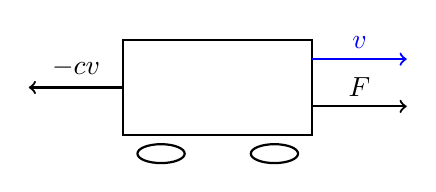
\begin{tikzpicture}[scale=1.2]
        % Draw the car as a rectangle
        \draw[thick] (0,0) rectangle (2,1);
        % Wheels
        \draw[thick] (0.4,-0.2) ellipse (0.25 and 0.1);
        \draw[thick] (1.6,-0.2) ellipse (0.25 and 0.1);
        % Forces
        \draw[->,thick] (2,0.3) -- ++(1,0) node[midway, above] {$F$};
        \draw[->,thick] (0,0.5) -- ++(-1,0) node[midway, above] {$-cv$};
        % Velocity arrow
        \draw[->,thick,blue] (2.0,0.8) -- ++(1,0.0) node[midway, above] {$v$};
    \end{tikzpicture}
    \caption{Free body diagram of a car}
    \label{f:car_fbd}
\end{figure}
\noindent Applying Newton's second law, the sum of forces is equal to mass times acceleration:
\begin{equation}
  m\dot{v} = F - cv
\end{equation}
where $m$ is the mass of the car, $F$ is the force generated by the tires, and $-cv$ is the linear drag. In this case to make the system first order we simply leave acceleration as $\dot{v}$ instead of $\ddot{x}$ where x would be the position of the vehicle. Rearranging, we obtain the standard first-order linear differential equation:
\begin{equation}
  \dot{v} + \frac{c}{m}v = \frac{F}{m}
\end{equation}
This equation describes the velocity dynamics of the car under a linear drag assumption. In this case $\sigma = c/m$ and $F = cf$. With these substitutions you arrive at the same equation as \ref{e:first_order}.

\subsubsection{Example Second Order System Formulation}

A second order system undergoing free motion will have dynamics that look like this
\begin{equation}\label{e:second_order}
\ddot{q} + 2\zeta \omega_n \dot{q} + {\omega_n}^2 = {\omega_n}^2 f
\end{equation}
where $q$ is a generalized coordinate, $\sigma$ is the inverse of the time constant $\tau$, f is the forcing function, $\omega_n$ is the natural frequency of the system and $\zeta$ is the damping ratio. Examples of these types of systems include mass, spring dampers in linear translation as well as torsional systems and penduluums. Anything that oscillates will exhibit this behavior. 

\subsubsection{Second Order Equations of Motion for a Mass Spring Damper System}

A mass-spring-damper system is a classic example of a second-order system. The system consists of a mass $m$ attached to a spring with spring constant $k$ and a damper with damping coefficient $c$. The mass is free to move along a single axis $x$, and the system is subject to an external force $f$ as shown in Figure \ref{f:msd}.

\begin{figure}[H]
    \centering
    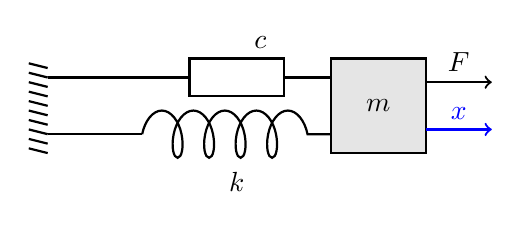
\begin{tikzpicture}[scale=1.2]
        % Draw the wall
        \draw[thick] (-1,.2) -- (0,0.2);
        \draw[thick] (-1,0.8) -- (0,0.8);
        \foreach \y in {0,0.1,...,1.0}
            \draw[thick] (-1,\y) -- (-1.2,\y+0.05);

        % Draw the spring
        \draw[thick,decorate,decoration={coil,aspect=0.5,segment length=4mm,amplitude=3mm}] (0,0.2) -- (2,0.2);

        % Draw the damper
        \draw[thick] (0,0.8) -- (0.5,0.8);
        \draw[thick] (0.5,1.0) rectangle (1.5,0.6);
        \draw[thick] (1.5,0.8) -- (2.0,0.8);

        % Draw the mass
        \draw[thick,fill=gray!20] (2,0) rectangle (3,1.0);

        % Labels
        \node at (2.5,0.5) {$m$};
        \node[above] at (1.25,1.0) {$c$};
        \node[below] at (1,-0.1) {$k$};
        \draw[->,thick,blue] (3.0,0.25) -- ++(0.7,0) node[midway, above] {$x$};
        \draw[->,thick] (3.0,0.75) -- ++(0.7,0) node[midway, above] {$F$};
    \end{tikzpicture}
    \caption{Mass-spring-damper system}
    \label{f:msd}
\end{figure}

Consider the mass-spring-damper system depicted above. The spring exerts a restoring force $-kx$ that is always directed opposite to the displacement $x$ of the mass from equilibrium, while the damper exerts a resistive force $-c\dot{x}$ proportional and opposite to the velocity $\dot{x}$. The external force $F(t)$ acts in the direction of motion. According to Newton's second law, the sum of these forces acting on the mass equals the mass times its acceleration, leading to the equation 
\begin{equation}
m\ddot{x} = F - c\dot{x} - kx 
\end{equation}
Rearranging terms, we obtain the standard form of the equation of motion for the mass-spring-damper system.
\begin{equation}
\ddot{x} + \frac{c}{m}\dot{x} + \frac{k}{m}x = \frac{F}{m}
\end{equation}
This second-order linear differential equation fully describes the dynamic response of the system to any external force $F$. Looking at equation \ref{e:second_order} we can see that $\omega_n = \sqrt{k/m}$ and $\zeta = c/(2\sqrt{mk})$. Furthermore, if we let $F = kf$ we arrive at the same equation as \ref{e:second_order}.

\subsection{Solutions to Differential Equations}

The differential equations presented in the previous section can be solved using a variety of methods. The most common methods are the characteristic and particular solution method and the Laplace transform method. The sections below will discuss both methods starting with the characteristic and particular solution method.

\subsubsection{Characteristic and Particular Solutions for First Order Systems}

First the first order system defined above will be solved first. For a first order linear differential equation of the form presented in equation \ref{e:first_order}, the general solution is the sum of the homogeneous (characteristic) solution and a particular solution. The particular solution corresponds to the steady-state response when the forcing function $f$ is constant. In this case assume $f$ is a step function which is just a constant $f_0$. The particular solution $q_p(t)=C$ where $C$ is a constant and thus $\dot{q_p}=\dot{C}=0.$ Plugging this into equation \ref{e:first_order} gives
\begin{equation}
    0 + \sigma q_p = \sigma f_0 
\end{equation}
Thus, the particular solution for a constant input is simply $q_p = f_0$. If the forcing function is not constant then the particular solution will be a function of time and solving for the particular solution will be more difficult. Examples of this include sinusoidal forcing functions or exponentially decaying forcing functions. The solutions to these types of forcing functions can be found in many differential equations textbooks and will not be discussed here for the time being. The homogeneous solution is found by setting the forcing function to zero and solving the resulting equation assuming that $q_h(t)=Ae^{st}$. Thus, the homogeneous equation is
\begin{equation}
    \dot{q_h} + \sigma q_h = Ase^{st} + \sigma Ae^{st} = Ae^{st}(s+\sigma) = 0
\end{equation}
In the equation above the result yields 3 equations that could be equal to zero. The first is $A=0$ which is a trivial solution and thus not considered. The second is $e^{st}=0$ which is never true for any real or complex value of s. The third is $s+\sigma=0$ which is the charactertic equation for the first order system. The solution to this equation yields the characteristic root $s=-\sigma$. Thus, the homogeneous solution is
\begin{equation}
    q_h(t) = Ae^{-\sigma t}
\end{equation}
where A is a constant determined by the initial conditions. The general solution is the sum of the homogeneous and particular solutions
\begin{equation}
    q(t) = q_h(t) + q_p(t) = Ae^{-\sigma t} + f_0
\end{equation}
The constant A can be determined by the initial condition $q(0)=q_0$ which yields
\begin{equation}
    q(0) = A + f_0 = q_0 \implies A = q_0 - f_0
\end{equation}
Thus, the final solution to the first order system is 
\begin{equation}
    q(t) = q_0 - f_0 + Ae^{-\sigma t}
\end{equation}
or more simply
\begin{equation}
    q(t) = f_0 + (q_0 - f_0)e^{-\sigma t}
\end{equation}
In the case of the car example the solution would be
\begin{equation}
    v(t) = \frac{F_0}{c} + \left(v_0 - \frac{F_0}{c}\right)e^{-\frac{c}{m}t}
\end{equation}
noting that $\sigma = c/m$,$F_0 = cf_0$ and $v_0$ is the initial velocity of the car. Typically for these types of systems the initial velocity is zero so the equation simplifies to
\begin{equation}
    v(t) = \frac{F_0}{c}\left(1 - e^{-\frac{c}{m}t}\right)
\end{equation}
which shows that the car will asymptotically approach a steady state velocity of $F_0/c$. This will be plotted later in the time response section for open loop analysis.

\subsubsection{Characteristic and Particular Solutions for Second Order Systems}

\subsubsection{Laplace Solutions}

\subsection{Time Response of First and Second Order Systems}

\subsection{Proportional Derivative Integral Control}

\subsection{Lyapunov Control}

\subsection{Sliding Mode Control}

\subsection{Adaptive Control}

\subsection{Controllability}

Controllability is formally stated as a system where any initial
state $x(0)=x_0$ and final state $x_1,t_1>0$, there exists a piecewise
continuous input $u(t)$ such that $x(t_1)=x_1$. 
For a fixed wing aircraft the system has 12 states with 8 dynamic
modes and 4 zero or rigid body modes. For a fixed wing aircraft the system has 12 states with 8 dynamic
modes and 4 zero or rigid body modes. A conventional aircraft has 4
controls to control these 12 modes. The easiest way to test the 
controllability of a system  is to compute the
controllability matrix. However, the controllability matrix must be
computed using a linearized model such that
$\dot{\vec{x}}=A\vec{x}+B\vec{u}$. In order to do this the aircraft
must be in equilibrium. For this example the aircraft is
set with an initial velocity of $20~m/s$ at an altitude of
$200~m$. The altitude command is set to $200~m$ and the heading
command is set to zero. Given the zero heading angle command and the
symmetry of the configurations investigated the rudder and aileron
commands are set to zero. Thus, only the thrust and elevator controls
are activated for the trimming procedure. Each configuration is
simulated for 200 seconds or until the derivatives of all states
except $\dot{x}$ are within a required tolerance. Using this
equilibrium point a linear model can be computed by using forward
finite differencing assuming that the
aircraft model is put in the form $\dot{\vec{x}} = F(\vec{x},\vec{u})$.
\begin{equation}
\dot{\vec{\delta x}} = \frac{F(\vec{x_0}+\Delta \vec{x_0},\vec{u_0})-F(\vec{x_0},\vec{u_0})}{\Delta
  \vec{x}}\vec{\delta x} + \frac{F(\vec{x_0},\vec{u_0}+\Delta
  \vec{u})-F(\vec{x_0},\vec{u_0})}{\Delta \vec{u}}\vec{\delta u}
\end{equation}
This linear model is the classic linear model where
$\dot{\vec{\delta x}}=A\vec{\delta{x}}+B\vec{\delta{u}}$. Using this linear model, the
controllability matrix can be computed as
\begin{equation}
W_C = [B~AB~A^2B~A^3B~...~A^{N-1}B]
\end{equation}
where N is the number of states in the system. With the controllability
matrix formulated, the rank of the matrix is computed. If the
$rank(W_C)=N$ the system is said to be controllable.

